\documentclass[
  captions=tableheading,
  bibliography=totoc, 
  titepage=firstiscover,
]{scrartcl}

\usepackage{blindtext} %neuer input

\usepackage{longtable} % Tabellen über mehrere Seiten

\usepackage[utf8]{inputenc} %neuer input

\usepackage{scrhack}

\usepackage[aux]{rerunfilecheck} %Warnung falls nochmal kompiliert werden muss

\usepackage{fontspec} %Fonteinstellungen

\recalctypearea{}

\usepackage[main=ngerman]{babel} %deutsche Spracheinstellung

\usepackage{ragged2e} %neuer input

\usepackage{amsmath, nccmath}

\usepackage{amssymb} %viele mathe Symbole

\usepackage{mathtools} %Erweiterungen für amsmath


\DeclarePairedDelimiter{\abs}{\lvert}{\rvert}
\DeclarePairedDelimiter{\norm}{\lVert}{\rVert}

\DeclarePairedDelimiter{\bra}{\langle}{\rvert}
\DeclarePairedDelimiter{\ket}{\lvert}{\rangle}

\DeclarePairedDelimiterX{\braket}[2]{\langle}{\rangle}{
#1 \delimsize| #2
}

\NewDocumentCommand \dif {m}
{
\mathinner{\symup{d} #1}
}


\usepackage[
  math-style=ISO,
  bold-style=ISO,
  sans-style=italic,
  nabla=upright,
  partial=upright,
  warnings-off={
    mathtools-colon,
    mathtools-overbracket,
  },
]{unicode-math}

\setmathfont{Latin Modern Math}
\setmathfont{XITS Math}[range={scr, bfscr}]
\setmathfont{XITS Math}[range={cal, bfcal}, StylisticSet=1]


\usepackage[
  locale=DE,
  separate-uncertainty=true,
  per-mode=reciprocal,
  output-decimal-marker={,},
]{siunitx}

\usepackage[autostyle]{csquotes} %richtige Anführungszeichen

\usepackage{xfrac}

\usepackage{float}

\floatplacement{figure}{htbp}

\floatplacement{table}{htbp}

\usepackage[ %floats innerhalb einer section halten
  section,   %floats innerhalb er section halten
  below,     %unterhalb der Section aber auf der selben Seite ist ok
]{placeins}

\usepackage[
  labelfont=bf,
  font=small,
  width=0.9\textwidth,
]{caption}

\usepackage{subcaption} %subfigure, subtable, subref

\usepackage{graphicx}

\usepackage{grffile}

\usepackage{booktabs}

\usepackage{microtype} %Verbesserungen am Schriftbild

\usepackage[
backend=biber,
]{biblatex}

\addbibresource{../lit.bib}

\usepackage[ %Hyperlinks im Dokument
  german,
  unicode,
  pdfusetitle,
  pdfcreator={},
  pdfproducer={},
]{hyperref}

\usepackage{bookmark}

\usepackage[shortcuts]{extdash}

%\usepackage{warpcol}

\usepackage{physics}
\allowdisplaybreaks

\begin{document}
    \title{Physik IV Übungsblatt 7}
    \author{  
    Tobias Rücker\\
    \texorpdfstring{\href{mailto:tobias.ruecker@tu-dortmund.de}{tobias.ruecker@tu-dortmund.de}
    \and}{,} 
    Paul Störbrock\\
    \texorpdfstring{\href{mailto:paul.stoerbrock@tu-dortmund.de}{paul.stoerbrock@tu-dortmund.de}}{}
    }
\maketitle
\center{\Large Abgabegruppe: \textbf{4H}}
\thispagestyle{empty}

\newpage
\tableofcontents
\thispagestyle{empty}
\newpage

\setcounter{page}{1}

\section{Aufgabe 1}

    \begin{figure}[H]
        \centering
        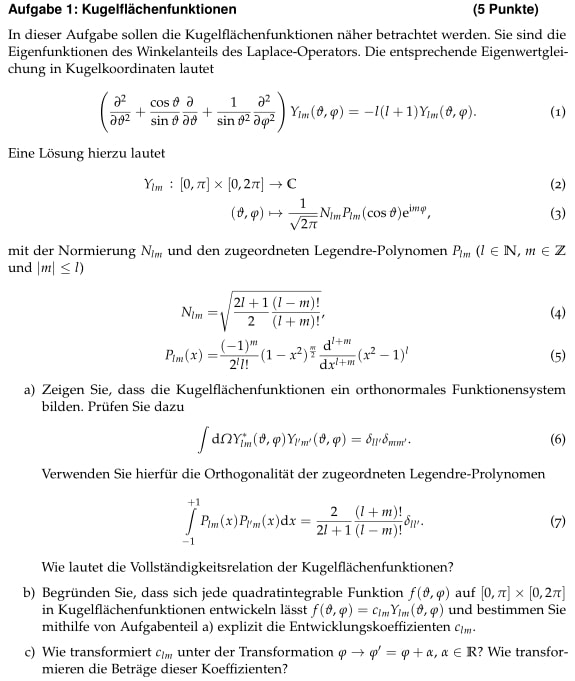
\includegraphics[width=\textwidth]{images/Aufgabe1.jpg}
        \label{fig:1}
    \end{figure}

    \subsection{a)}
    \begin{align}
    &\int \dif{\omega} Y_{lm}^* (\theta, \phi) Y_{l'm'}(\theta , \phi)\\
    &=\int \dif{\omega} \frac{1}{\sqrt{2 \pi}} N_{lm} P_{lm} (\cos \theta) e^{-im\phi} 
    \frac{1}{\sqrt{2 \pi}} N_{l'm'} P_{l'm'}(\cos \theta) e^{im' \phi}\\
    &=\int \dif{\omega} \frac{1}{2 \pi} N_{lm} N_{l'm'} e^{i(m'-m)\phi} P_{lm} P_{l'm'}\\
    &=\int_0^{\pi} \int_0^{2 \pi} \frac{1}{2 \pi} N_{lm} N_{l'm'} \sin \theta e^{i(m'-m)\phi} P_{lm} P_{l'm'}
    \dif{\phi} \dif{\theta}\\
    &=\int_0^{\pi} \frac{1}{2\pi} N_{lm} N_{l'm'} \sin \theta P_{lm} P_{l'm'} \frac{1}{i(m'-m)} 
    \underbrace{(e^{i(m'-m)2 \pi}-1 )}_{=0} \dif{\theta} \\
    \intertext{
        für alle $m \ne m'$ 
        Fall $m=m'$
    }
    &=\int_0^{\pi} \int_0^{2 \pi} \frac{1}{2 \pi} N_{lm} N_{l'm} P_{lm} P_{l'm} \sin \theta e^{i(m-m)\phi} \dif{\phi} \dif{\theta}\\
    &= \int_0^{\pi} N_{lm} N_{l'm} P_{lm} P_{l'm} \sin \theta \dif{\theta} \\
    \Rightarrow &\int_0^{2\pi} \frac{1}{2 \pi} \frac{1}{2\pi} e^{i(m'-m)\phi} = \delta _{mm'}\\
    &=\int_0^{\pi} N_{lm} N_{l'm} P_{lm} P_{l'm} \underbrace{\sin \theta}_{-\frac{\dif{\cos \theta}}{\dif{\theta}}} \dif{\theta}\\
    &= \int_{\pi}^0 N_{lm} N_{l'm} P_{lm}(\cos \theta) P_{l'm} (\cos \theta) \dif{\cos \theta}\\
    \intertext{
        Substitution 
    }    
    x&= \cos \theta\\
    \frac{\dif{x}}{\dif{\cos \theta}} &=1\\
    \intertext{
        weiter
    }
    &= \int _{-1}^1 N_{lm} N_{lm'} P_{lm}(x) P_{l'm}(x) \dif{x}\\
    &= N_{lm} N_{l'm} \frac{2}{2l+1} \frac{(l+m)!}{(l-m)!} \delta _{ll'} \\
    &=\begin{cases}
    l=l' \;1\\
    l \ne l' \;0
    \end{cases}\\
    &\Rightarrow \int \dif{\omega} Y_{l'm'}^* Y_{lm} = \delta_{ll'} \delta _{mm'}\\
    &\sum_{l=0}^{\infty} \sum_{m=-l}^l Y_{lm}^* (\theta ' , \phi ') Y_{lm} (\theta , \phi) = \delta (\phi - \phi ') \delta (\cos \theta - \cos \theta ')\\
    \end{align}

    \subsection{b)}
    \begin{align}
    \intertext{
        \flushleft{Die\,}\justifying Kugelflächenfunktionen bilden ein orthonormales Funktionensystem. Durch ihre Vollständigkeit 
        bilden sie einen Satz von quadratintegrablen Funktionen im $L^2$ und können alle anderen Funktionen in $L^2$ darstellen.
    }
    c_{lm} &= \int_0^{2 \pi} \int_0^\pi Y_{lm}^* f(\theta, \phi) \sin \theta \dif{\theta} \dif{\phi} \\
    \end{align}

    \subsection{c)}
    \begin{align}
        c_{lm} &= \int_0^{2 \pi} \int_0^\pi Y_{lm}^* f(\theta, \phi) \sin \theta \dif{\theta} \dif{\phi} \\
        \intertext{
            Transformation:
        }
        \phi ' &= \phi + \alpha \\
        \phi &= \phi ' - \alpha \\
        \frac{\dif{\phi}}{\dif{\phi '}} &=1\\
        \intertext{
            weiter
        }
        c_{lm} &= \int_0^{2 \pi} \int_0^{\pi} Y_{lm}^* (\theta , \phi '-\alpha) f(\theta , \phi '  - \alpha) \sin \theta \dif{\theta} \dif{\phi '}\\
        &= \int_0^{2 \pi} \int_0^{\pi} \frac{1}{\sqrt{2 \pi}} N_{lm} P_{lm} (\cos \theta) e^{-i m (\phi ' - \alpha)} d_{lm} \frac{1}{\sqrt{2 \pi}} N_{lm} P_{lm} (\cos{\theta}) e^{im(\phi ' + \alpha)}\\
        &= \int_0^{2 \pi} \frac{1}{2 \pi} \underbrace{\int_0^{\pi}  (P_{lm} (\cos \theta))^2}_{=1} e^{im 2 \alpha} d_{lm}\\
        &= e^{im2 \alpha} d_{lm}\\
        d_{lm} &= e^{-im2 \alpha} c_{lm}\\
        \abs{c_{lm}} &= \abs{e^{im 3 \alpha} c_{lm}} \\
        &=\sqrt{(e^{-im2 \alpha} d_{lm}^*)(e^{im2 \alpha} d_{lm})} \\
        \abs{c_{lm}} &= \abs{d_{lm}}
        \intertext{
            \flushleft{Die\,}\justifying Beträge bleiben bei der Transformation erhalten, während sich die normalen Koeffizienten um 
            eine Phase $\alpha$ unterscheiden.
        }
    \end{align}



\section{Aufgabe 2}

    \begin{figure}[H]
        \centering
        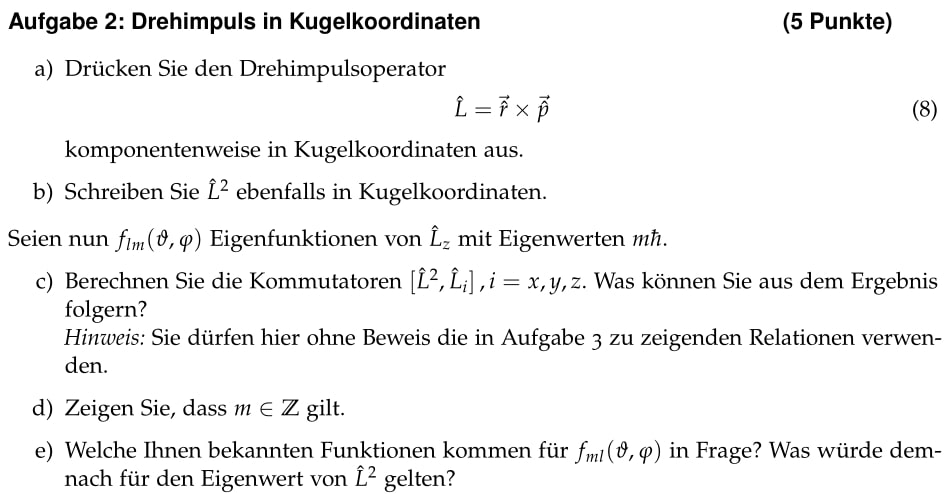
\includegraphics[width=\textwidth]{images/Aufgabe2.jpg}
        \label{fig:2}
    \end{figure}

    \subsection{a)}

    \begin{align*}
    \vec{\hat{L}} &= \vec{\hat{r}} \times \vec{\hat{p}}\\
    L_x &= (yp_z-zp_y)\\
    L_y &= (zp_x-xp_z)\\
    L_z &= (xp_y-yp_x)\\
    \tilde{\vec{r}} &= 
    \begin{pmatrix}
        r\cos(\varphi)\sin(\theta)\\
        r\sin(\varphi)\sin(\theta)\\
        r\cos(\theta)
    \end{pmatrix}\\
    p_x &= -\text{i} \hbar \frac{\partial}{\partial x}\\
    p_y &= -\text{i} \hbar \frac{\partial}{\partial y}\\
    p_z &= -\text{i} \hbar \frac{\partial}{\partial z}
    \intertext{
        \flushleft{Einsetzen\;}\justifying in $L_{x,y,z}$:
    }
    L_x &= -\text{i} \hbar(y\frac{\partial}{\partial z}-z\frac{\partial}{\partial y})\\
    L_y &= -\text{i} \hbar(z\frac{\partial}{\partial x}-x\frac{\partial}{\partial z})\\
    L_z &= -\text{i} \hbar(x\frac{\partial}{\partial y}-y\frac{\partial}{\partial x})\\
    \\
    \frac{\partial \tilde{\vec{r}}}{\partial \varphi} &= \frac{\partial \vec{r}}{\partial x} (-r\sin(\varphi))\sin(\theta) + \frac{\partial \vec{r}}{\partial y} r\cos(\varphi)\sin(\theta)\\
    &= -y \frac{\partial \vec{r}}{\partial x} + x \frac{\partial \vec{r}}{\partial y}\\
    \Phi' &=
    \begin{pmatrix}
        \cos(\varphi)\sin(\theta) & -r\sin(\varphi)\sin(\theta) & r\cos(\varphi)\cos(\theta)\\
        \sin(\varphi)\sin(\theta) & r\cos(\varphi)\sin(\theta) & r\sin(\varphi)\cos(\theta)\\
        \cos(\theta) & 0 & -r\sin(\theta)
    \end{pmatrix}\\
    (\Phi')^{-1} &= \frac{1}{\text{det}|\Phi'|}\text{adj}(\Phi')\\
    &= \frac{1}{(-r^2\sin(\theta)} 
    \begin{pmatrix}
        -r^2\cos(\varphi)\sin^2(\theta) & -r^2\sin(\varphi)\sin^2(\theta) & -r^2\cos(\varphi)\sin(\theta)\\
        r\sin(\varphi) & -r\cos(\varphi) & 0\\
        -c\cos(\varphi)\sin(\theta)\cos(\theta) & -r\sin(\varphi)\sin(\theta)\cos(\theta) & r\sin^2(\theta)
    \end{pmatrix}\\
    &= 
    \begin{pmatrix}
        \cos(\varphi)\sin(\theta) & \sin(\varphi)\sin(\theta) & \cos(\theta)\\
        -\frac{\sin(\varphi)}{r\sin(\theta)} & \frac{\cos(\varphi)}{r\sin(\theta)} & 0\\
        \frac{\cos(\varphi)\cos(\theta)}{r} & \frac{\sin(\varphi)\cos(\theta)}{r} & \frac{-\sin(\theta)}{r}\\
    \end{pmatrix}\\
    \Rightarrow \frac{\partial}{\partial x} &= \cos(\varphi)\sin(\theta)\frac{\partial}{\partial r} - \frac{\sin(\varphi)}{r\sin(\theta)}\frac{\partial}{\partial \varphi} + \frac{\cos(\varphi)\cos(\theta)}{r}\frac{\partial}{\partial \theta}\\
    \Rightarrow \frac{\partial}{\partial y} &= \sin(\varphi)\sin(\theta)\frac{\partial}{\partial r} + \frac{\cos(\varphi)}{r\sin(\theta)}\frac{\partial}{\partial \varphi} + \frac{\sin(\varphi)\cos(\theta)}{r}\frac{\partial}{\partial \theta}\\
    \Rightarrow \frac{\partial}{\partial z} &= \cos(\theta)\frac{\partial}{\partial r} -\frac{\sin(\theta)}{r}\frac{\partial}{\partial \theta}
    \intertext{
        \flushleft{Einsetzen\;}\justifying in $L_{x,y,z}$:
    }
    L_x &= -\text{i} \hbar(y\frac{\partial}{\partial z}-z\frac{\partial}{\partial y})\\
    &= -\text{i} \hbar\left(r\sin(\varphi)\sin(\theta) % muss noch gesplitted werden! (von hier)
    \left(\cos(\theta)\frac{\partial}{\partial r} - \frac{\sin(\theta)}{r}\frac{\partial}{\partial \theta}\right)
    -r\cos(\theta) \left(\sin(\varphi)\sin(\theta)\frac{\partial}{\partial r} + \frac{\cos(\varphi)}{r\sin(\theta)}\frac{\partial}{\partial \varphi} 
    + \frac{\sin(\varphi)\cos(\theta)}{r}\frac{\partial}{\partial \theta}\right)\right)\\ % (bis hier)
    &= -\text{i}\hbar \left( -\sin(\varphi)\frac{\partial}{\partial\theta} - \frac{\cos(\varphi)}{\tan(\theta)}\frac{\partial}{\partial\varphi}\right)\\
    &= \text{i}\hbar \left( \sin(\varphi)\frac{\partial}{\partial\theta} + \frac{\cos(\varphi)}{\tan(\theta)}\frac{\partial}{\partial\varphi}\right)\\
    \\
    L_y &= -\text{i} \hbar(z\frac{\partial}{\partial x}-x\frac{\partial}{\partial z})\\
    &= -\text{i} \hbar\left(r\cos(\theta)  % muss noch gesplitted werden! (von hier)
    \left(\cos(\varphi)\sin(\theta)\frac{\partial}{\partial r} - \frac{\sin(\varphi)}{r\sin(\theta)}\frac{\partial}{\partial \varphi} + \frac{\cos(\theta)\cos(\varphi)}{r}\frac{\partial}{\partial \theta}\right)
    -r\cos(\varphi)\sin(\theta) 
    \left(\cos(\theta)\frac{\partial}{\partial r} - \frac{\sin(\theta)}{r}\frac{\partial}{\partial \theta}\right) \right)\\ % (bis hier)
    &= \text{i}\hbar\left( -\cos(\varphi)\frac{\partial}{\partial \theta} + \frac{\sin(\varphi)}{\tan(\theta)}\frac{\partial}{\partial \varphi} \right)\\
    \\
    L_z &= (xp_y-yp_x)\\
    &= \text{i}\hbar\frac{\partial}{\partial \varphi}
    \end{align*}


    \subsection{b)}

    \begin{align*}
    &\begin{pmatrix}
        \text{i}\hbar \left( \sin(\varphi)\frac{\partial}{\partial\theta} + \frac{\cos(\varphi)}{\tan(\theta)}\frac{\partial}{\partial\varphi}\right)\\
        \text{i}\hbar \left( -\cos(\varphi)\frac{\partial}{\partial\theta} + \frac{\sin(\varphi)}{\tan(\theta)}\frac{\partial}{\partial\varphi}\right)\\
        \text{i}\hbar\frac{\partial}{\partial \varphi}
    \end{pmatrix}
    \begin{pmatrix}
        \text{i}\hbar \left( \sin(\varphi)\frac{\partial}{\partial\theta} + \frac{\cos(\varphi)}{\tan(\theta)}\frac{\partial}{\partial\varphi}\right)\\
        \text{i}\hbar \left( -\cos(\varphi)\frac{\partial}{\partial\theta} + \frac{\sin(\varphi)}{\tan(\theta)}\frac{\partial}{\partial\varphi}\right)\\
        \text{i}\hbar\frac{\partial}{\partial \varphi}
    \end{pmatrix}\\
    &= -\hbar \left( \sin^2(\varphi)\frac{\partial^2}{\partial \theta^2} + \frac{\cos(\varphi)\sin(\varphi)}{\tan(\theta)} \frac{\partial^2}{\partial \varphi \partial \theta} %muss noch gesplitted werden! (von hier)
    - \frac{\sin(\varphi)\cos(\theta)}{\sin^2(\theta)} \frac{\partial}{\partial \varphi} + \frac{\cos(\varphi)\cos(\varphi)}{\tan(\theta)} \frac{\partial}{\partial \theta}
    + \frac{\cos(\varphi)\sin(\varphi)}{\tan(\theta)}\frac{\partial^2}{\partial \varphi \partial \theta} + \frac{\cos^2(\varphi)}{\tan^2(\theta)} \frac{\partial^2}{\partial \varphi^2}
    - \frac{\cos(\varphi)\sin(\varphi)}{\tan(\theta)}\frac{\partial}{\partial \varphi} + \cos^2(\varphi) \frac{\partial^2}{\partial \theta^2}
    + \frac{\cos(\varphi)\sin(\varphi)}{\sin^2(\theta)}\frac{\partial}{\partial \varphi} - \frac{\cos(\varphi)\sin(\varphi)}{\tan(\theta)} \frac{\partial^2}{\partial \varphi \partial \theta}
    - \frac{\cos(\varphi)\sin(\varphi)}{\tan(\theta)} \frac{\partial^2}{\partial \varphi \partial \theta} + \frac{\sin^2(\varphi)}{\tan(\theta)} \frac{\partial}{\partial \theta}
    + \frac{\sin^2(\varphi)}{\tan^2(\theta)} \frac{\partial^2}{\partial \varphi^2} + \frac{\cos(\varphi)\sin(\varphi)}{\tan(\theta)} \frac{\partial}{\partial \varphi} + \frac{\partial^2}{\partial \varphi^2} \right)\\ % (bis hier)
    &= -\hbar \left( \frac{\partial^2}{\partial \theta^2} + \frac{1}{\tan(\theta)} \frac{\partial}{\partial \theta} + \frac{1}{\tan^2(\theta)} \frac{\partial^2}{\partial \varphi^2} + \frac{\partial^2}{\partial \varphi^2} \right)\\
    &= -\hbar \left( \frac{\partial^2}{\partial \theta^2} + \frac{1}{\tan(\theta)} \frac{\partial}{\partial \theta} + \frac{\partial^2}{\partial \varphi^2} \left( \frac{1}{\tan^2(\theta)} + 1 \right) \right)\\
    &= -\hbar \left( \frac{1}{\sin(\theta)} \frac{\partial}{\partial \theta} \left( \sin(\theta) \frac{\partial}{\partial \theta} \right) + \frac{1}{\sin(\theta)} \frac{\partial^2}{\partial \varphi^2} \right)
    \end{align*}

    \subsection{c)}

    \subsection{d)}

    \subsection{e)}


\section{Aufgabe 3}

    \begin{figure}[H]
        \centering
        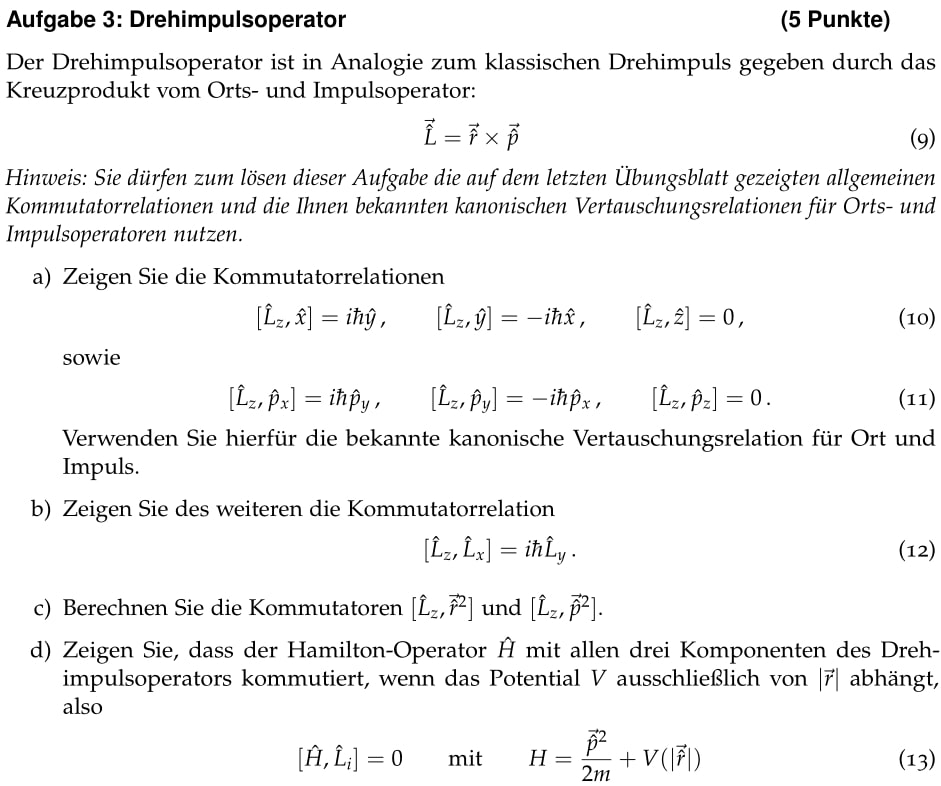
\includegraphics[width=\textwidth]{images/Aufgabe3.jpg}
        \label{fig:3}
    \end{figure}

    \subsection{a)}

    \begin{align*}
        \vec{\hat{L}} &= \vec{\hat{r}} \times \vec{\hat{p}}\\
        \vec{\hat{r}} &= 
        \begin{pmatrix}
            x\\
            y\\
            z
        \end{pmatrix},
        \qquad \vec{\hat{p}} = -\text{i}\hbar
        \begin{pmatrix}
            \frac{\partial}{\partial x}\\
            \frac{\partial}{\partial y}\\
            \frac{\partial}{\partial z}
        \end{pmatrix}\\
        \vec{\hat{L}} &= 
        \begin{pmatrix}
            L_x\\
            L_y\\
            L_z
        \end{pmatrix}
        = 
        -\text{i}\hbar
        \begin{pmatrix}
            y\frac{\partial}{\partial z} - z\frac{\partial}{\partial y}\\
            z\frac{\partial}{\partial y} - x\frac{\partial}{\partial z}\\
            x\frac{\partial}{\partial y} - y\frac{\partial}{\partial x}
        \end{pmatrix}\\
        \\
        \left[ L_z,x \right]\Psi &= -\text{i}\hbar L_z\cdot x - x \cdot \left( -\text{i}\hbar L_z \right)\Psi = -\text{i}\hbar \left( L_z\cdot x - x \cdot L_z \right)\Psi\\
        &= -\text{i}\hbar \left( \left( x\frac{\partial}{\partial y} - y\frac{\partial}{\partial x} \right)x - x \left( x\frac{\partial}{\partial y} - y\frac{\partial}{\partial x} \right) \right)\Psi\\
        &= -\text{i}\hbar \left( \underbrace{x\frac{\partial}{\partial y}x}_{=0} - \underbrace{y\frac{\partial}{\partial x}x}_{=y} - \underbrace{x^2\frac{\partial}{\partial y}}_{=0} + \underbrace{xy\frac{\partial}{\partial x}}_{=0} \right)\Psi\\
        &= -\text{i}\hbar y\Psi\\
        \\
        \left[ L_z,y \right]\Psi &= -\text{i}\hbar \left( L_z\cdot y - y \cdot L_z \right) \Psi\\
        &= -\text{i}\hbar \left( \left( x\frac{\partial}{\partial y} - y\frac{\partial}{\partial x} \right)y - y\left( x\frac{\partial}{\partial y} - y\frac{\partial}{\partial x} \right) \right)\Psi\\
        &= -\text{i}\hbar \left( \underbrace{x\frac{\partial}{\partial y}y}_{=x} - \underbrace{y\frac{\partial}{\partial x}y}_{=0} - \underbrace{xy\frac{\partial}{\partial y}}_{=0} + \underbrace{y^2\frac{\partial}{\partial x}}_{=0} \right)\Psi\\
        &= -\text{i}\hbar x\Psi\\
        \\
        \left[ L_z,z \right]\Psi &= -\text{i}\hbar \left( L_z\cdot z - z \cdot L_z \right) \Psi\\
        &= -\text{i}\hbar \left( \left( x\frac{\partial}{\partial y} - y\frac{\partial}{\partial x} \right)z - z\left( x\frac{\partial}{\partial y} - y\frac{\partial}{\partial x} \right) \right)\\
        &= -\text{i}\hbar \left( \underbrace{x\frac{\partial}{\partial y}z}_{=0} - \underbrace{y\frac{\partial}{\partial x}z}_{=0} - \underbrace{xz\frac{\partial}{\partial y}}_{=0} + \underbrace{yz\frac{\partial}{\partial x}}_{=0} \right)\\
        &= 0\\
        \\
        \left[ L_z,p_x \right]\Psi &= \left( -\text{i}\hbar \right)^2 \left(L_z\cdot \frac{\partial}{\partial x} - \frac{\partial}{\partial x} \cdot L_z\right)\Psi\\
        &= \left( -\text{i}\hbar \right)^2 \left( \left( x\frac{\partial}{\partial y} - y\frac{\partial}{\partial x} \right) \frac{\partial}{\partial x} -\frac{\partial}{\partial x} \left( x\frac{\partial}{\partial y} - y\frac{\partial}{\partial x} \right) \right)\Psi\\
        &= \left( -\text{i}\hbar \right)^2 \left( x\frac{\partial}{\partial y}\frac{\partial}{\partial x} - y\frac{\partial}{\partial x}\frac{\partial}{\partial x} - \underbrace{\frac{\partial}{\partial x}x \frac{\partial}{\partial y}}_{!} + \frac{\partial}{\partial x}y \frac{\partial}{\partial x} \right)\Psi\\
        &\frac{\partial}{\partial x} \frac{\partial}{\partial y} x\Psi \stackrel{!}{=} \frac{\partial}{\partial y}\Psi + x\frac{\partial}{\partial x}\Psi \frac{\partial}{\partial y} = \left( \frac{\partial}{\partial y} + x\frac{\partial}{\partial x} \frac{\partial}{\partial y} \right) \Psi\\
        &= \left( -\text{i}\hbar \right)^2 \left( x\frac{\partial}{\partial y}\frac{\partial}{\partial x} - y\frac{\partial}{\partial x}\frac{\partial}{\partial x} - \underbrace{\frac{\partial}{\partial y} - x\frac{\partial}{\partial x} \frac{\partial}{\partial y}}_{!} + \frac{\partial}{\partial x}y \frac{\partial}{\partial x} \right)\Psi\\
        &= \left( -\text{i}\hbar \right)^2 \frac{-\partial}{\partial y}\Psi\\
        &= \text{i}\hbar \hat{p}_y \Psi\\
        \\
        \left[ L_z,p_y \right]\Psi &= \left( -\text{i}\hbar \right)^2 \left( L_z\cdot \frac{\partial}{\partial y} - \frac{\partial}{\partial y} \cdot L_z \right) \Psi\\
        &= \left( -\text{i}\hbar \right)^2 \left( \left( x\frac{\partial}{\partial y} - y\frac{\partial}{\partial x} \right) \frac{\partial}{\partial y} - \frac{\partial}{\partial y} \left( x\frac{\partial}{\partial y} - y\frac{\partial}{\partial x} \right) \right)\Psi\\
        &= \left( -\text{i}\hbar \right)^2 \left( x\frac{\partial}{\partial y} \frac{\partial}{\partial y} - y\frac{\partial}{\partial x} \frac{\partial}{\partial y} - \frac{\partial}{\partial y} x\frac{\partial}{\partial y} + \underbrace{\frac{\partial}{\partial y} y\frac{\partial}{\partial x}}_{! (\text{siehe oben})} \right)\Psi\\
        &= \left( -\text{i}\hbar \right)^2 \left( x\frac{\partial}{\partial y} \frac{\partial}{\partial y} - y\frac{\partial}{\partial x} \frac{\partial}{\partial y} - \frac{\partial}{\partial y} x\frac{\partial}{\partial y} + \underbrace{\frac{\partial}{\partial x} + y\frac{\partial}{\partial y} \frac{\partial}{\partial x}}_{!} \right)\Psi\\
        &= \left( -\text{i}\hbar \right)^2 \frac{\partial}{\partial x}\Psi\\
        &= \text{i}\hbar \hat{p}_x \Psi\\
        \\
        \left[ L_z,p_z \right]\Psi &= \left( -\text{i}\hbar \right)^2 \left( L_z\cdot \frac{\partial}{\partial z} - \frac{\partial}{\partial z} \cdot L_z \right)\Psi\\
        &= \left( -\text{i}\hbar \right)^2 \left( \left( x\frac{\partial}{\partial y} - y\frac{\partial}{\partial x} \right) \frac{\partial}{\partial z} - \frac{\partial}{\partial z} \left( x\frac{\partial}{\partial y} - y\frac{\partial}{\partial x} \right) \right)\Psi\\
        &= \left( -\text{i}\hbar \right)^2 \left( x\frac{\partial}{\partial y} \frac{\partial}{\partial z} - y\frac{\partial}{\partial x} \frac{\partial}{\partial z} - \frac{\partial}{\partial z}x\frac{\partial}{\partial y} + \frac{\partial}{\partial z}y\frac{\partial}{\partial x} \right)\Psi\\
        &= 0\\
    \end{align*}

    \subsection{b)} 

    \begin{align*}
        \left[ \hat{L}_z,\hat{L}_x \right] &= -\text{i}\hbar \left(\left( x\frac{\partial}{\partial y} - y\frac{\partial}{\partial x} \right) \left( y\frac{\partial}{\partial z} - z\frac{\partial}{\partial y} \right) - \left( y\frac{\partial}{\partial z} - z\frac{\partial}{\partial y} \right) \left( x\frac{\partial}{\partial y} - y\frac{\partial}{\partial x} \right)\right)\\
        &= -\text{i}\hbar \left( x \underbrace{\frac{\partial}{\partial y}y}_{=1} \frac{\partial}{\partial z} - \underbrace{x\frac{\partial}{\partial y} z\frac{\partial}{\partial y}}_{=0} - \underbrace{y\frac{\partial}{\partial x} y\frac{\partial}{\partial z}}_{=0} + \underbrace{y\frac{\partial}{\partial x} z\frac{\partial}{\partial y}}_{=0} 
        - \underbrace{y\frac{\partial}{\partial z} x\frac{\partial}{\partial y}}_{=0} + \underbrace{y\frac{\partial}{\partial z} y\frac{\partial}{\partial x}}_{=0} + \underbrace{z\frac{\partial}{\partial y} x\frac{\partial}{\partial y}}_{=0} - z \underbrace{\frac{\partial}{\partial y}y}_{=1} \frac{\partial}{\partial x}\right)\\
        &= -\text{i} \hbar\left(x\frac{\partial}{\partial z}-z\frac{\partial}{\partial x}\right)\\
        &= \text{i} \hbar \left(z\frac{\partial}{\partial x}-x\frac{\partial}{\partial z}\right)\\
        &= \text{i}\hbar \hat{L}_y
    \end{align*}

    \subsection{c)}

    \begin{align*}
        \vec{\hat{r}}^2 &= \left( x^2+y^2+z^2 \right), \qquad \vec{\hat{p}}^2 = \left(\frac{\partial^2}{\partial x^2}+\frac{\partial^2}{\partial y^2}+\frac{\partial^2}{\partial z^2} \right)\\
        \left[ \hat{L}_z,\vec{\hat{r}}^2 \right] \Psi &= -\text{i}\hbar \left( x\frac{\partial}{\partial y} - y\frac{\partial}{\partial x} \right) \left( x^2+y^2+z^2 \right) - \left( x^2+y^2+z^2 \right) \left(-\text{i}\hbar \left( x\frac{\partial}{\partial y} - y\frac{\partial}{\partial x} \right)\right)\Psi\\
        &= -\text{i}\hbar \left(\left( x\frac{\partial}{\partial y} - y\frac{\partial}{\partial x} \right) \left( x^2+y^2+z^2 \right) - \left( x^2+y^2+z^2 \right) \left( x\frac{\partial}{\partial y} - y\frac{\partial}{\partial x} \right)\right)\Psi\\
        &= \left( \left[ L_z,x \right]x - x\left[ L_z,x \right] + \left[ L_z,y \right]y - y\left[ L_z,y \right] + \underbrace{\left[ L_z,z \right]}_{=0}z - z\underbrace{\left[ L_z,z \right]}_{=0}\right) \Psi\\
        &= \left( \text{i}\hbar \hat{y}\hat{x} - \hat{x}\text{i}\hbar\hat{y} - \text{i}\hbar \hat{x}\hat{y} + \hat{y}\text{i}\hbar\hat{x} \right) \Psi\\
        &= 2\text{i}\hbar \left( \hat{y}\hat{x}-\hat{x}\hat{y} \right) \Psi\\
        &= 2\text{i}\hbar \underbrace{\left[ \hat{y},\hat{x} \right]}_{=0} \Psi = 0\\
        \\
        \left[ \hat{L}_z,\vec{\hat{p}}^2 \right] \Psi &= -\text{i}\hbar \left(\left( x\frac{\partial}{\partial y} - y\frac{\partial}{\partial x} \right) \left(\frac{\partial^2}{\partial x^2}+\frac{\partial^2}{\partial y^2}+\frac{\partial^2}{\partial z^2} \right) - \left(\frac{\partial^2}{\partial x^2}+\frac{\partial^2}{\partial y^2}+\frac{\partial^2}{\partial z^2} \right) \left( x\frac{\partial}{\partial y} - y\frac{\partial}{\partial x} \right)\right)\Psi\\
        &= \left( \left[ L_z,\hat{p}_x^2 \right] + \left[ L_z,\hat{p}_y^2 \right] + \left[ L_z,\hat{p}_z^2 \right] \right)\Psi\\
        &= \left( \left[ L_z,\hat{p}_x \right]\hat{p}_x - \hat{p}_x\left[ L_z,\hat{p}_x \right] + \left[ L_z,\hat{p}_y \right]\hat{p}_y - \hat{p}_y\left[ L_z,\hat{p}_y \right] + \underbrace{\left[ L_z,\hat{p}_z \right]}_{=0}\hat{p}_z - \hat{p}_z\underbrace{\left[ L_z,\hat{p}_z \right]}_{=0}\right) \Psi\\
        &= -\text{i}\hbar\left( \text{i}\hbar \hat{p}_y\hat{p}_x - \hat{p}_x\text{i}\hbar\hat{p}_y - \text{i}\hbar \hat{p}_x\hat{p}_y + \hat{p}_y\text{i}\hbar\hat{p}_x \right) \Psi\\
        &= 2\text{i}\hbar \underbrace{\left[ \hat{p}_y,x \right]}_{=0} \Psi = 0\\
    \end{align*}

    \subsection{d)}





\end{document}